\documentclass[a4paper,11pt]{article}
\usepackage[spanish]{babel}
\usepackage[margin=1in]{geometry}

\usepackage{hyperref}
\usepackage[xetex]{graphicx}
\usepackage{upquote}
\usepackage{listings}
\usepackage{wrapfig}

\usepackage{xcolor}
 
\definecolor{codegreen}{rgb}{0,0.6,0}
\definecolor{codegray}{rgb}{0.5,0.5,0.5}
\definecolor{codepurple}{rgb}{0.58,0,0.82}
\definecolor{backcolour}{rgb}{0.95,0.95,0.92}
 
\lstdefinestyle{mystyle}{
    backgroundcolor=\color{backcolour},   
    commentstyle=\color{codegreen},
    keywordstyle=\color{magenta},
    numberstyle=\tiny\color{codegray},
    stringstyle=\color{codepurple},
    basicstyle=\ttfamily\footnotesize,
    breakatwhitespace=false,         
    breaklines=true,                 
    captionpos=b,                    
    keepspaces=true,                 
    numbers=left,                    
    numbersep=5pt,                  
    showspaces=false,                
    showstringspaces=false,
    showtabs=false,                  
    tabsize=2
}
 
\lstset{style=mystyle}

%\usepackage{csquotes}
%\usepackage[backend=biber,style=nature]{biblatex}
%\addbibresource{citations.bib}

\begin{document}

\begin{center}
    {\huge\bfseries Aprendizaje de Máquinas Avanzado}\\[3mm]
    {\Large\bfseries Módulo 0}\\[3mm]
    {\Large Felipe Tobar \& Taco de Wolff}\\
    {\normalsize\textit{Centro de Modelamiento Matemático, Universidad de Chile}}\\
\end{center}

En este módulo, que es parte del curso Aprendizaje de Máquinas Avanzado, vamos a verificar que todos tienen Python y las librerías requeridas. Todo debe funcionar antes del comienzo de las clases, en que comenzamos con módulo 1.

\section{Instalar Python y librerías requeridos}

\begin{wrapfigure}{R}[0pt]{0.25\textwidth}
    \vspace{-10pt}
    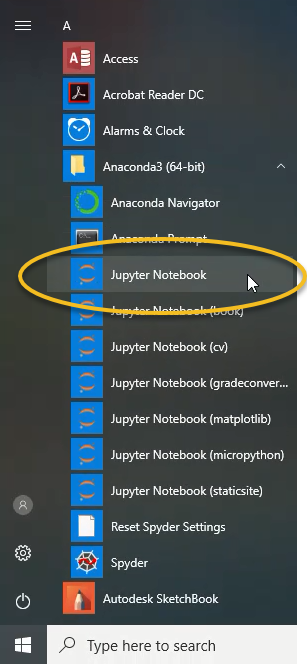
\includegraphics[width=0.25\textwidth]{windows_start_jupyter_notebook.png}
    \vspace{-50pt}
\end{wrapfigure}

Si ya tienes Python 3.6 o 3.7 instalado, pasa a la siguiente seción. Fíjese que necesitas estas librerías instaladas: \texttt{numpy, scipy, matplotlib, jupyter, pandas, pytorch}.

Si no tienes Python instalado, les recomendamos instalar Anaconda, que contiene todo que necesitamos. Descarga desde \url{https://www.anaconda.com/distribution/} la última versión (sería Python 3.7) y sigue con la instalación. Después, se ve el \emph{Jupyter Notebook} como en la imagen a la derecha.

\section{Preparar flujo de trabajo}
Para tener una mejor manera de trabajar, ocuparemos un flujo de trabajo que se baja en Jupyter Notebook. Los Notebooks nos ayudan a correr los códigos más fácil, presentar lo que creaste en una manera más visuál, y mejora la distribución de los códigos. Para empezar inicie la aplicación Jupyter Notebook. Una pantalla en tu browser se abrirá y es la que ocuperamos desde ahora.

Navegue hacia la carpeta donde quieres guardar los datos del curso. Ahí presione en \emph{New} y elija \emph{Python 3} para crear un nuevo notebook. Escriba \texttt{print('Hola mundo')} y ejecute presionando Shift+Enter. También puedes iniciar presionando el butón \emph{Run} que es indicado por azul en la imagen abajo. Con el más (+) puedes agregar una nueva celda (indicado por rojo).

\begin{figure}[ht]
\centering
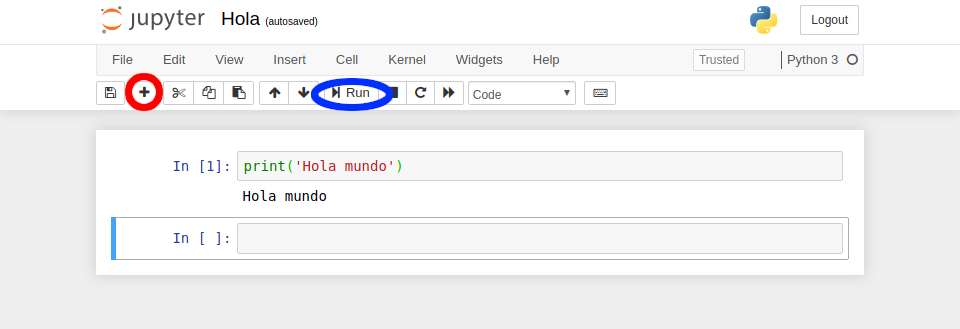
\includegraphics[scale=1.75]{jupyter.png}
\end{figure}

\section{Experimentar con Python y las librerías}
Abra el notebook que acompaña este documento y sigue con las instrucciónes allí.

%\printbibliography
\end{document}
